%%%%%%%%%%%%%%%%%%%%%%%%%%%%%%%%%%%%%%%%%
% Stylish Article
% LaTeX Template
% Version 2.1 (1/10/15)
%
% This template has been downloaded from:
% http://www.LaTeXTemplates.com
%
% Original author:
% Mathias Legrand (legrand.mathias@gmail.com) 
% With extensive modifications by:
% Vel (vel@latextemplates.com)
%
% License:
% CC BY-NC-SA 3.0 (http://creativecommons.org/licenses/by-nc-sa/3.0/)
%
%%%%%%%%%%%%%%%%%%%%%%%%%%%%%%%%%%%%%%%%%

%========================================================================================
\documentclass[fleqn,11pt]{SelfArx}
\usepackage[english]{babel} % Specify a different language here - english by default
%----------------------------------------------------------------------------------------
%-----------------------------------------------------------------------------------------------
\usepackage[english]{babel}
\usepackage[squaren,cdot]{SIunits}
\usepackage{amsmath,amsthm}
\usepackage{CormorantGaramond}
\usepackage{xspace}
%-----------------------------------------------------------------------------------------------


%----------------------------------------------------------------------------------------
%-----------------------------------------------------------------------------------------------
\setlength{\abovecaptionskip}{4pt}
\setlength{\columnsep}{5.5mm}
\setlength{\columnseprule}{0.2pt}
\setlength{\fboxrule}{0.4pt} % Width of the border around the abstract
%-----------------------------------------------------------------------------------------------
\definecolor{color1}{RGB}{0,0,90} % Color of the article title and sections
\definecolor{color2}{RGB}{0,20,20} % Color of the boxes behind the abstract and headings
\definecolor{color3}{RGB}{0,0,192} % Color of the article title and sections
%-----------------------------------------------------------------------------------------------
\usepackage[hyperindex,breaklinks]{hyperref} % Required for hyperlinks
\hypersetup{%
    hidelinks,
    colorlinks,
    breaklinks=true,
    urlcolor=color3,
    citecolor=color1,
    linkcolor=color1,
    bookmarksopen=false,
    pdftitle={Title},
    pdfauthor={Author}
}
%-----------------------------------------------------------------------------------------------
\newtheorem{example}{Example}
%-----------------------------------------------------------------------------------------------

%----------------------------------------------------------------------------------------
%-----------------------------------------------------------------------------------------------
\makeatletter
\immediate\write18{datelog > \jobname.info}
\makeatother
%-----------------------------------------------------------------------------------------------
% Journal information
\JournalInfo{engrXiv}
\Archive{\input{\jobname.info}revision}
% Article title
\PaperTitle{On Illustrating Carnot's General Proposition by Means of Reversible Stirling Engines}
\Authors{%
    C.~Naaktgeboren\textsuperscript{1$\star$},
    K.~A.~É.~Beck\textsuperscript{2},
    J-M.~S.~Lafay\textsuperscript{3}
}
\affiliation{%
    \textsuperscript{1}%
    \textit{%
        Universidade Tecnológica Federal do Paraná -- UTFPR, Câmpus Guarapuava.
        Grupo de Pesquisa em Ciências Térmicas.
}}
\affiliation{%
    \textsuperscript{2}%
    \textit{%
        Universidade Tecnológica Federal do Paraná -- UTFPR, Câmpus Pato Branco.
        Programa de Pós-Graduação em Engenharia Elétrica -- PPGEE.
}}
\affiliation{%
    \textsuperscript{3}%
    \textit{%
        Universidade Tecnológica Federal do Paraná -- UTFPR, Câmpus Pato Branco.
        Programa de Pós-Graduação em Engenharia Elétrica -- PPGEE.
}}
\affiliation{%
    \textsuperscript{$\star$}%
    \textbf{Corresponding  author}: NaaktgeborenC$\cdot$PhD@gmail$\cdot$com
}
\Keywords{%
    Carnot principles ---
    Carnot general proposition ---
    Second law of Thermodynamics ---
    Reversible Stirling engine models ---
    Thermal efficiency
}
\newcommand{\keywordname}{Keywords}
\Highlights{%
    Highlight1 ---
    Highlight2 ---
    etc...
}
\newcommand{\highlightname}{Highlights}
%-----------------------------------------------------------------------------------------------
\Abstract{%
    Carnot's general proposition, also referred to as one of Carnot's  principles,  states  that
    the  work  producing  potential  of  heat---harvested  by   reversible   heat   engines---is
    \emph{independent} on the working fluid  and  on  engine  internal  details,  being  only  a
    function of the temperatures of the reservoirs with which the engine  exchanges  heat.  This
    concept,  usually  presented  to  ME  students  in  the  context  of  the  second   law   of
    thermodynamics,  is  usually  proven  by  contradiction,  using  second  law  concepts   and
    abstractions, without concrete examples, even though Carnot's proposition mentions  concrete
    things such as working fluids and engine internal details. This work  proposes  to  document
    the usage of reversible Stirling engine models that take the engine  arrangement  and  fluid
    properties into account towards demonstrating the validity of Carnot's general  proposition,
    as to be referred to opportunely, for instance, whenever a concrete example is requested.
}
%-----------------------------------------------------------------------------------------------

%========================================================================================
\begin{document}
%========================================================================================
\flushbottom % Makes all text pages the same height
\maketitle % Print the title and abstract box
\tableofcontents % Print the contents section
\thispagestyle{empty} % Removes page numbering from the first page
%----------------------------------------------------------------------------------------
%-----------------------------------------------------------------------------------------------
\section{Introduction}

    The subject of the second law  of  thermodynamics  figures  amidst  the  most  philosophical
    teaching topics in mechanical engineering. Many studies have been produced around the  theme
    of pedagogical improvements in presenting the second law of thermodynamics, under a  variety
    of    strategies~\cite{1995-MoukalledF+NuwayhidRY-IJMEE,     1996-KaufmanR+SheldonE-AmJPhys,
    1997-BejanA-IJMEE,              1997-DunbarWR+LiorN-IJMEE,               2011-LewinsJ-IJMEE,
    2015-BeaubouefSr-IntJMechEngEduc}.

    One of the key concepts covered  in  textbook  presentations  of  the  second  law  are  the
    so-called          Carnot          principles~\cite{2013-CengelYA+BolesMA-AMGH}           or
    corolaries~\cite{2002-MoranMJ+ShapiroHN-LTC}, or  claim~\cite[p.~88]{2006-BejanA-Wiley},  or
    even deductions than make up  one  principle~\cite{1986-JonesJB+HawkinsGA-Wiley}---different
    sources attribute different names and list a varying number of what Carnot has mostly called
    \emph{propositions}~\cite{1897-ThurstonRH-Wiley}, without labeling them, except for the ones
    that he named ``fundamental'' and ``general''.

    Carnot's fundamental proposition is a statement of a necessary condition for heat engines to
    attain ``maximum'' work production from heat~\cite[p.~56]{1897-ThurstonRH-Wiley}:

    \begin{quote}
        \it
        ``[...] that in the bodies employed to realize the motive  power
        of heat there should not occur any change of  temperature  which
        may not be due to a change of volume.''
    \end{quote}

    Recall his work appears many  years  before  the  second  law  of  thermodynamics  had  been
    established, and the properties we now use, such as entropy, had been  invented.  In  modern
    terms, Carnot's fundamental proposition can be  paraphrased  as  ``the  temperature  of  the
    working fluid can only change during isentropic changes in  volume'',  recalling  that  both
    friction and heat transfer irreversibilities would cause the fluid to experience temperature
    changes that could not be explained by adiabatic and reversible change in volume.

    Carnot's general proposition, on the other hand, is the generalization  of  his  fundamental
    proposition, and states that~\cite[p.~68]{1897-ThurstonRH-Wiley}:

    \begin{quote}
        \it
        ``The motive power of heat is independent of the agents employed
        to realize it; its quantity is fixed solely by the  temperatures
        of the bodies between, which is effected, finally, the  transfer
        of the caloric.''
    \end{quote}

    Meaning, in current thermodynamic terms, that the maximum work producing potential  of  heat
    is independent of the working fluid substance employed in its production,  being  determined
    only by the temperatures\footnote{Note the plural which embeds what would later on  make  up
    the Kelvin-Planck statement of the second law.} in which heat is  being  transfered.  Modern
    texts make it explicit that such  work  producing  potential  is  also  independent  on  the
    engine's internal details~\cite{2013-CengelYA+BolesMA-AMGH}, or, equivalently,  sequence  of
    processes~\cite{2002-MoranMJ+ShapiroHN-LTC} of the reversible machines.

    Carnot's general proposition is typically presented to mechanical  engineering  students  in
    the context of the second law of thermodynamics in the form of a  statement  followed  by  a
    proof   by    contradiction~\cite{2013-CengelYA+BolesMA-AMGH,    2002-MoranMJ+ShapiroHN-LTC,
    1986-JonesJB+HawkinsGA-Wiley},  using  second  law  concepts  and  abstractions,  i.e.,   by
    proposing a violation of the general proposition and showing in the conceptual realm that it
    leads to a violation of a statement of the second law of thermodynamics---a method  that  is
    both sufficient and general from a mathematical viewpoint.

    Despite the mathematical fitness of this approach, it lacks concrete examples. In one  hand,
    one may argue that lack of concrete examples may  pose  unnecessary  extra  difficulties  on
    learners; on the other hand, the proposition's phrasing seems to beg for concrete  examples,
    as it mentions concrete things such as working fluids and engine internal details.

    Keen and attentive learners may correctly wonder that both heat intake and net  work  output
    done by reversible models of different real engines may be written as complicated  functions
    of the engines' internal details, working fluid properties, and reservoir temperatures---and
    wonder how all these things may fit together under  the  restrictions  of  Carnot's  general
    proposition.

    This work focuses in documenting one such analysis, and thus becoming a reference  that  can
    be  presented  opportunely---not  in  place  of,  but   alongside   the   usual   proof   by
    contradiction---to inquiring  learners,  or  whenever  an  instructor  see  to  be  fitting.
    Moreover, it is hoped that the concrete aspects of Carnot's general proposition are met,  at
    least in the few instances provided herein.

    Well-known engineering textbook reversible cycles include (i)~the Carnot, (ii)~the Stirling,
    and (iii)~the Ericson  ones~\cite{2013-CengelYA+BolesMA-AMGH}.  The  Stirling  cycle  is  of
    peculiar interest for the task due to (i)~the present time interest  displayed  towards  it;
    (ii)~the fact that many reversible models are available in  the  literature;  and  (iii)~the
    existence of three different such engine configuration types: the $\alpha$-,  $\beta$-,  and
    $\gamma$-ones---so that variations on engine internal details and operating  parameters  and
    on working  fluid  can  be  performed  in  the  context  of  illustrating  Carnot's  general
    proposition.

    Historically,   reversible    Stirling    engine    cycles    have    been    proposed    by
    Schmidt~\cite{1871-SchmidtG-ZeitVerDeutschIng},                                             
    Finkelstein~\cite{1960-FinkelsteinT-SAEIntl},   Walker~\cite{1962-WalkerG-JMechEngSci}   and
    Kirkley~\cite{1962-KirkleyDW-JMechEngSci}. The focus of early works has  been  investigating
    optimal engine construction and operating parameters.

    More recently, Cheng and Yang~\cite{2012-ChengCH+YangHS-ApEnergy}  developed  a  reversible,
    dimensionless, and parametric Stirling engine model that accounts not only for working fluid
    and for engine operating parameter variations, but also for engine configuration alteration,
    i.e., among the $\alpha$-, the $\beta$-, and  the  $\gamma$-types.  Moreover,  they  provide
    exact analytical expressions for net work output and for heat  inlet  that  are  written  in
    terms of the various model parameters and engine internal configurations.

    This work uses Cheng and Yang's model~\cite{2012-ChengCH+YangHS-ApEnergy} in producing  more
    concrete examples of the validity of Carnot's general proposition than the  usual  proof  by
    contradiction, that may be of interest to engineering students learning the  second  law  of
    thermodynamics.

%-----------------------------------------------------------------------------------------------


%----------------------------------------------------------------------------------------
%-----------------------------------------------------------------------------------------------
\section{Reversible Stirling Engine Model}

    In     this     section,     Cheng     and     Yang's     reversible     Stirling     engine
    model~\cite{2012-ChengCH+YangHS-ApEnergy} is presented as an  example  for  the  purpose  of
    illustrating the validity of Carnot's general proposition. Owing to  the  context  in  which
    such example is regarded useful, i.e., in teaching the second law of thermodynamics, only  a
    concise subset of the model that is useful for the stated goal is  being  presented,  as  to
    avoid unnecessary distractions.

    Moreover, the model nomenclature  is  kept  the  same  as  the  one  used  in  the  original
    reference~\cite{2012-ChengCH+YangHS-ApEnergy}, so as to  allow  curious  readers  to  easily
    lookup in the original work the parts abridged in this work. There is only a  minute  change
    in nomenclature employed herein for conciseness, which  consists  in  annotating  the  greek
    letter of the engine configuration above a symbol, so as to specify that symbol's expression
    for that particular engine configuration, starting on Eq.~(\ref{eq:Ve}).

    \begin{figure}[ht]
        \centering
        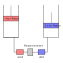
\includegraphics[width=0.8\columnwidth]{fig/stirling_engine_alpha_color.pdf}
        \caption{Schematic representation of an ideal Stirling engine of the $\alpha$-type.  The
            `eHX'  and  the  `cHX'  are  the  `expansion'  and  `compression'  heat  exchangers,
            respectively of high- and low- temperatures. The power pistons and  the  regenerator
            are indicated.}
        \label{fig:alpha}
    \end{figure}

    Let $V_{cs}$ and $V_{es}$ be piston and displacer  sweep  volumes  in  the  operation  of  a
    reversible Stirling engine of either $\alpha$-,  $\beta$-,  or  $\gamma$-type---in  Stirling
    engine nomenclature, it is common to name high- and low-  temperature  spaces  and  adjacent
    moving       parts       as        `expansion',        and        `compression'        ones,
    respectively~\cite{2013-CengelYA+BolesMA-AMGH}; hence the `$c$' and  `$e$'  subscripts.  Let
    further $V_d$ be the so-called engine ``dead volume'',  which  is  composed  by  piston  and
    displacer minimum clearances and regenerator volumes, i.e., $V_d =  V_{emin}  +  V_{cmin}  +
    V_r$, respectively.

    \begin{figure}[ht]
        \centering
        \includegraphics[width=0.8\columnwidth]{fig/stirling_engine_beta_color.pdf}
        \caption{Schematic representation of an ideal Stirling engine of the  $\beta$-type.  The
            `eHX'  and  the  `cHX'  are  the  `expansion'  and  `compression'  heat  exchangers,
            respectively of high- and low- temperatures. The power and displacement pistons  and
            the regenerator are indicated.}
        \label{fig:alpha}
    \end{figure}

    Let $\phi$ be the engine's crankshaft angle, and $\alpha$  be  the  expansion-to-compression
    piston-piston  (for  the  $\alpha$-type)  or  piston-displacer   (for   the   $\beta$-   and
    $\gamma$-types)  phase  angle.  For  all  engine  configurations   the   expansion   volume,
    $V_e(\phi)$, is:
    %
    \begin{align}
        \label{eq:Ve}
        V_e(\phi) &= V^{\alpha}_e(\phi) = V^{\beta}_e(\phi) = V^{\gamma}_e(\phi) \nonumber\\
                  &= V_{emin} + \frac{1}{2} V_{es}(1 + \sin(\phi + \alpha)).
    \end{align}

    The compression volume, $V_c(\phi)$, is configuration dependent:
    %
    \begin{align}
        \label{eq:Vca}
        V^{\alpha}_c(\phi) &= V_{cmin} + \frac{1}{2} V_{es} \kappa (1 + \sin(\phi)), \\
        \label{eq:Vcb}
        V^{\beta}_c(\phi)  &= V_{cmin} +
            \frac{1}{2} V_{es} (\sqrt{1 - 2\kappa\cos\alpha + \kappa^2} \nonumber\\
                           &+ \kappa\sin\phi - \sin(\phi + \alpha)), \\
        \label{eq:Vcg}
        V^{\gamma}_c(\phi) &= V_{cmin} + \frac{1}{2} V_{es}
            (1 + \kappa + \kappa\sin\phi \nonumber\\
                           &- \sin(\phi + \alpha)),
    \end{align}
    %
    \noindent where $\kappa \equiv V_{cs}/V_{es}$ is the engine sweep volume ratio.

    It is worth noting that each engine has its very own distinct volume dynamics,  making  them
    suitable to verifying Carnot's general proposition from the point  of  view  of  ``different
    internal details''.

    Let the total engine volume---the instantaneous volume  occupied  by  the  engine's  working
    fluid,
    %
    \begin{equation}
        V(\phi) = V_e(\phi) + V_c(\phi) + V_r,
    \end{equation}
    %
    \noindent be written in terms of  a  configuration  dependent  dimensionless  function  most
    generally written as $\Phi(\phi | \chi, \kappa,  \alpha)$,  i.e.,  in  terms  of  parameters
    $\chi$, $\kappa$ and $\alpha$, so that
    %
    \begin{equation}
        V(\phi) = V_{es}\Phi(\phi | \chi, \kappa, \alpha),
    \end{equation}
    %
    \noindent with:
    %
    \begin{align}
        \label{eq:Phia}
        \Phi^{\alpha}(\phi | \chi, \kappa, \alpha) &= \chi + \frac{1}{2}(1 + \kappa) \nonumber\\
            &+ \frac{1}{2}(\sin(\phi + \alpha) + \kappa\sin\phi),\\
        \label{eq:Phib}
        \Phi^{\beta}(\phi | \chi, \kappa, \alpha) &= \chi + \frac{1}{2}\kappa\sin\phi +
            \frac{1}{2}(1 \nonumber\\
            &+ \sqrt{1 - 2\kappa\cos\alpha + \kappa^2}),\\
        \label{eq:Phig}
        \Phi^{\gamma}(\phi | \chi, \kappa) &= \chi + \frac{1}{2}(2 + \kappa)
            + \frac{1}{2}\kappa\sin\phi.
    \end{align}
    %
    \noindent where $\chi \equiv V_{d}/V_{es}$ is the engine dead  volume  ratio.  It  is  worth
    noting that for the $\gamma$-type engine, parameter  $\alpha$  is  absent  from  the  $\Phi$
    function, thus showing that different  engine  configuration  may  also  lead  to  different
    mathematical ``signature'' of intermediate functions.

    The working fluid pressure, $p$, is assumed to be uniform throughout the engine  cavity---as
    pressure-drops would introduce  irreversibilities  that  would  prevent  one  from  checking
    Carnot's general proposition. Assuming, for the sake of simplicity, while still allowing for
    different fluids to be used, ideal gas $p$-$V$-$T$ behavior of the working fluid, one has:
    %
    \begin{equation}
        \label{eq:P}
        p = \frac{mR}{\frac{V_e}{T_e} + \frac{V_c}{T_c} + \frac{V_d}{T_d}}
          = \frac{mRT_e}{V_{es}}\Psi(\phi | \alpha, \kappa, \tau, \chi),
    \end{equation}
    %
    \noindent where $T_e$, $T_c$, and $T_d \equiv (T_e + T_c)/2$ are the expansion, compression,
    and dead space temperatures, respectively, with $T_e > T_c$ for heat engine  operation;  and
    $\Psi(\phi | \alpha, \kappa, \tau, \chi)$ is the dimensionless engine pressure  function  of
    $\phi$ with parameters $\alpha, \kappa, \tau, \chi$, in which $\tau \equiv T_c / T_e$ is the
    compression-to-expansion reservoir temperature ratio. It is worth noting  that  if  Carnot's
    general proposition is to hold, the thermal efficiency of the exemplified  Stirling  engines
    must be a function of $\tau$ only.

    The  dimensionless  pressure  function  is  a  multi-term,  engine   configuration dependent
    expression:
    %
    \begin{align}
        \label{eq:Psia}
        \frac{1}{\Psi^{\alpha}(\phi)} &=
                \frac{2\chi}{1 + \tau} +
                \frac{\kappa + \tau}{2\tau} +
                \frac{\kappa\sin\phi}{2\tau} \nonumber\\
            &+  \frac{\sin(\phi + \alpha)}{2},\\
        \label{eq:Psib}
        \frac{1}{\Psi^{\beta}(\phi)}  &=
                \frac{2\chi}{1 + \tau} +
                \frac{\tau + \sqrt{1 - 2\kappa\cos\alpha + \kappa^2}}{2\tau} \nonumber\\
            &+  \frac{\kappa\sin\phi}{2\tau} +
                \frac{(\tau - 1)\sin(\phi + \alpha)}{2\tau},\\
        \label{eq:Psig}
        \frac{1}{\Psi^{\gamma}(\phi)} &=
                \frac{2\chi}{1 + \tau} +
                \frac{1 + \tau + \kappa}{2\tau} +
                \frac{\kappa\sin\phi}{2\tau} \nonumber\\
            &+  \frac{(\tau - 1)\sin(\phi + \alpha)}{2\tau}.
    \end{align}

    The $RT_e$-normalized (i)~specific net cycle work, $\bar{W}$, and (ii)~specific inlet  cycle
    heat, $\bar{Q}_{in}$, are dimensionless quantities that can be expressed as:
    %
    \begin{align}
        \label{eq:W}
        \bar{W} &= \frac{\oint p\,\difff(V/m)}{RT_e} \nonumber\\
                &= \int_0^{2\pi} \Psi(\phi)
                   \frac{\partial\Phi(\phi | \chi, \kappa, \alpha)}{\partial\phi}\,\difff\phi,\\
        \label{eq:Q}
        \bar{Q}_{in} &= \frac{\oint p\,\difff(V_e/m)}{RT_e} \nonumber\\
                     &= \frac{1}{2} \int_0^{2\pi} \Psi(\phi)
                        \cos(\phi + \alpha) \,\difff\phi,
    \end{align}
    %
    \noindent where the  variable  and  parameter  dependencies  of  the  integrands  were  made
    explicit, recalling that $\Phi$ has a different  mathematical  signature  for  $\gamma$-type
    engines,      with      respect      to      the      $\alpha$-      and      $\beta$-types,
    Eq.~(\ref{eq:Phia})--(\ref{eq:Phig}).

    Equations~(\ref{eq:W}) and (\ref{eq:Q}) embody the argument made on the Introduction section
    of this work, meaning that both  cycle  net  work  and  cycle  inlet  heat  expressions  are
    \emph{complicated} and \emph{different} functions of engine's internal details---whether  in
    terms   of   $\alpha$-,   $\beta$-,   or   of   $\gamma$-type   configurations,   but   also
    construction/tuning parameters such as $\alpha$, $\kappa$, and $\chi$---and of  the  thermal
    reservoir temperatures, $\tau$.

%-----------------------------------------------------------------------------------------------


%----------------------------------------------------------------------------------------
\input{01-02-Section-03.tex}
%========================================================================================
%-----------------------------------------------------------------------------------------------
\section{Conclusions}

    Text...

%-----------------------------------------------------------------------------------------------


%----------------------------------------------------------------------------------------
%-----------------------------------------------------------------------------------------------
\section*{Conflict of Interest}

    The authors declare that there is no conflict of interest in this work.

%-----------------------------------------------------------------------------------------------


%----------------------------------------------------------------------------------------
%-----------------------------------------------------------------------------------------------
\section*{CRediT Author Statement}

    \textbf{CN:} Conceptualization, Methodology, Writing - Original Draft, Writing -  Review  \&
    Editing, Project administration. \textbf{KAEB:} Methodology, Investigation, Formal analysis,
    Writing - Original Draft (figures), Writing - Review \& Editing. \textbf{JMSL:} Methodology,
    Resources, Writing - Review \& Editing, Supervision, Funding acquisition.

%-----------------------------------------------------------------------------------------------


%----------------------------------------------------------------------------------------
%-----------------------------------------------------------------------------------------------
\section*{Acknowledgements}

    \textbf{KAEB}  and  \textbf{JMSL}  acknowledge  the  financial  support  in  part   by   the
    Coordination of Improvement of Higher Education Personnel -- Brazil (CAPES) -- Finance  Code
    001. National Council for Scientific and Technological Development (CNPq),  from  Foundation
    Araucária (FA) and from Financier of Studies and Projects (FINEP).

    \textbf{CN} received no specific grant from any funding agency in the  public,  private,  or
    not-for-profit sectors.

    \textbf{All} authors acknowledge the Federal University of Technology -- Paraná (UTFPR)  and
    the Federal Institute of Education, Science and Technology of  Santa  Catarina  (IFSC),  who
    contributed to this study in providing  human  resources,  laboratories,  and  institutional
    access to bibliography databases.

    To YHWH God be the glory!

%-----------------------------------------------------------------------------------------------


%----------------------------------------------------------------------------------------
%-----------------------------------------------------------------------------------------------
\bibliographystyle{plain}
\bibliography{bibfile}
%-----------------------------------------------------------------------------------------------

%========================================================================================
\end{document}
%========================================================================================
